\documentclass[12pt, a4paper]{article}

\usepackage[utf8]{inputenc}
\usepackage[T1]{fontenc}
\usepackage[brazil]{babel}
\usepackage{geometry}
\usepackage{graphicx}
\usepackage{booktabs}
\usepackage{caption}
\usepackage{subcaption}
\usepackage{hyperref}
\usepackage{amsmath}
\usepackage{float}
\usepackage{xcolor}
\usepackage{listings}
\usepackage{parskip}
\usepackage{array}

\geometry{margin=2.5cm}

\hypersetup{
    colorlinks=true,
    linkcolor=black,
    urlcolor=blue,
    citecolor=black
}

\lstset{
    basicstyle=\ttfamily\small,
    backgroundcolor=\color{gray!10},
    frame=single,
    breaklines=true,
    keywordstyle=\color{blue},
    commentstyle=\color{green!60!black},
}

% Marcador para conteúdo ainda pendente da frente de redes neurais.
\newcommand{\pendente}[1]{\textit{\textcolor{red}{[Pendente: #1]}}}

% ─────────────────────────────────────────────────────────────────────────────
\title{
    \textbf{Detecção e Segmentação de Copas de \textit{Cecropia}
    (Embaúba) em Ortomosaico de VANT}\\[0.4em]
    \large Duas abordagens: Visão Computacional Clássica e
    Redes Neurais (SAM 3 + YOLOv8)\\[0.6em]
    \large INE5443 — Reconhecimento de Padrões \\ UFSC
}
\author{Grupo 10 \\[0.3em]
\small Gabriel Arantes F. Gualda \quad Fábio H. A. Coelho \quad Nena A. Impanta\\
\small Augusto de H. V. Guerner \quad Eduardo G. de Lazari}
\date{Julho de 2026}
% ─────────────────────────────────────────────────────────────────────────────

\begin{document}

\maketitle
\tableofcontents
\newpage

\section{Introdução}

O conhecimento detalhado sobre árvores individuais — sua identificação,
distribuição espacial e desenvolvimento ao longo do tempo — constitui base
fundamental para a pesquisa botânica, o manejo florestal e a conservação da
biodiversidade (Wielgosz et al., 2024; Fassnacht et al., 2016). Tradicionalmente,
essas informações são obtidas por inventários de campo que, embora eficazes,
apresentam custos elevados, complexidade logística e demanda por mão de obra
especializada, limitando a frequência e a escala em que podem ser conduzidos
(Ferretti et al., 2024). Essa limitação torna-se ainda mais relevante diante do
compromisso global da Década da Restauração de Ecossistemas (2021–2030), que
amplia a demanda por ferramentas capazes de acompanhar a evolução de áreas
florestais de forma eficiente (De Almeida et al., 2020).

Nesse contexto, os Veículos Aéreos Não Tripulados (VANTs) consolidaram-se como
ferramenta de alta relevância para o monitoramento florestal. Imagens com
resolução espacial na ordem de centímetros viabilizam a observação de
características morfológicas individuais das plantas — formato e coloração das
copas, padrões de ramificação e textura foliar — em nível de detalhe inviável com
imagens de satélite convencionais (Soltani et al., 2025). Contudo, a
disponibilidade de imagens de alta resolução, por si só, não resolve o problema do
monitoramento em larga escala: a análise visual de ortomosaicos por especialistas
torna-se inviável quando a área de estudo se amplia para dezenas ou centenas de
hectares.

Este trabalho aborda o problema da detecção e segmentação de copas de
\textit{Cecropia pachystachya} (embaúba) em um ortomosaico de VANT por meio de
\textbf{duas frentes complementares}:

\begin{itemize}
    \item \textbf{Parte I — Visão Computacional Clássica.} Um pipeline sem
    aprendizado profundo, baseado em segmentação por espaço de cor HSV, operações
    morfológicas, extração de contornos e filtros geométricos. É interpretável,
    auditável e computacionalmente leve, servindo como \textit{baseline} e como
    primeira estimativa da distribuição espacial da espécie.

    \item \textbf{Parte II — Redes Neurais (SAM 3 + YOLOv8).} Um pipeline
    semi-automatizado que integra o modelo fundacional de segmentação
    Segment Anything Model 3 (SAM 3) com o detector YOLOv8, reduzindo o esforço de
    anotação manual por meio de uma estratégia de ``curadoria por exclusão'' e
    permitindo detecção e segmentação individuais das copas em escala.
\end{itemize}

Ambas as frentes operam sobre o \textbf{mesmo ortomosaico} do experimento MataDIV
(mesma área, mesmo sistema de referência e mesma resolução espacial), o que
permite comparar diretamente as duas estratégias. A abordagem clássica evidencia
até onde é possível chegar com regras explícitas de cor e forma, enquanto a
abordagem neural mostra os ganhos e os custos de incorporar aprendizado de máquina
ao problema.

A espécie-alvo, \textit{Cecropia pachystachya} Trécul (Urticaceae), é uma árvore
pioneira de rápido crescimento, amplamente distribuída nas florestas tropicais e
subtropicais da região Neotropical (Berg et al., 2005). Ecologicamente, sua
presença e abundância estão associadas à intensidade de perturbações florestais,
o que a estabelece como indicadora do estágio de regeneração de uma área (Guitet
et al., 2018). Além disso, apresenta características morfológicas que favorecem sua
detecção em imagens aéreas — folhas grandes e palmatilobadas, coloração
verde-prateada na face abaxial e copa de arquitetura umbeliforme distinta das
demais espécies do dossel (Carvalho, 2008). A conjunção entre relevância ecológica
e distinguibilidade visual motivou sua escolha como modelo biológico para este
estudo.

\section{Objetivos}

\subsection*{Objetivo geral}

Desenvolver e avaliar metodologias para detecção e segmentação individual de copas
de \textit{Cecropia pachystachya} em ortomosaico de VANT, comparando uma abordagem
de visão computacional clássica com uma abordagem de redes neurais que integra o
SAM 3 e o YOLOv8, com ênfase na redução do esforço manual.

\subsection*{Objetivos específicos}

\begin{itemize}
    \item Construir um pipeline clássico interpretável (HSV, morfologia,
    contornos e filtros geométricos) e avaliá-lo quanto a precisão, recall e
    custo computacional.
    \item Desenvolver um pipeline semi-automatizado de detecção e segmentação com
    SAM 3, minimizando as etapas manuais de criação do dataset e treinamento do
    modelo.
    \item Avaliar o desempenho do pipeline neural na detecção e segmentação de
    copas de \textit{C. pachystachya} em diferentes cenários de composição
    florestal do experimento MataDIV.
    \item Discutir a replicabilidade das duas abordagens para a detecção e
    segmentação de outras espécies arbóreas.
\end{itemize}

\section{Área de Estudo e Coleta de Dados}
\label{sec:area}

\subsection{Área de estudo}

O estudo foi conduzido no experimento MataDIV (Mata Atlântica Diversidade),
localizado na Estação Experimental de Ciências Florestais de Itatinga, pertencente
à Escola Superior de Agricultura ``Luiz de Queiroz'' (ESALQ/USP), no município de
Itatinga, São Paulo, Brasil (23\textdegree06'S, 48\textdegree39'W). O MataDIV é um
experimento de diversidade arbórea e funcionamento ecossistêmico (BEF) integrado à
rede global TreeDivNet, plantado em 2019 em uma área de antigo talhão comercial de
\textit{Eucalyptus} (Verheyen et al., 2016; Paquette et al., 2018).

O experimento manipula três variáveis (riqueza de espécies, fertilização e
disponibilidade hídrica) em 144 parcelas experimentais que ocupam aproximadamente
8 hectares. Cada parcela possui dimensões de 20~m $\times$ 23~m e contém 100
árvores plantadas em espaçamento de 2,3~m, totalizando cerca de 14.400 indivíduos.
As composições combinam seis espécies nativas de estratégias ecológicas
contrastantes em 12 estratos distintos — de monoculturas a uma composição de alta
diversidade com 20 espécies. A \textit{Cecropia pachystachya} está presente em
cinco dessas composições, com densidade que varia de 100 indivíduos por parcela na
monocultura a aproximadamente 5 indivíduos nas parcelas de alta diversidade. Essa
variedade torna o MataDIV particularmente adequado para avaliar a robustez das
metodologias sob diferentes condições de complexidade do dossel.

\subsection{Coleta de dados e ortomosaico}
\label{sec:ortomosaico}

O sobrevoo foi realizado em 13 de março de 2026 com o VANT DJI Matrice 4T,
equipado com câmera RGB wide (sensor CMOS 1/1.3'', 48~MP, distância focal
equivalente a 24~mm, campo de visão de 82\textdegree). A coleta ocorreu a 23~m
acima do nível do solo, com sobreposição frontal e lateral de 80\%, resultando em
uma resolução espacial no solo (GSD) de aproximadamente 0,85~cm/pixel. As imagens
foram processadas por fotogrametria digital no software Agisoft Metashape,
gerando um ortomosaico georreferenciado de 48.264 $\times$ 47.029 pixels, com
quatro bandas espectrais (R, G, B e alfa), aproximadamente 8,46~GB em GeoTIFF,
projetado em SIRGAS 2000 / UTM zona 22S (EPSG:31982).

Esse único ortomosaico é a base de dados comum às duas frentes deste trabalho. A
diferença entre elas está na forma como o ortomosaico é recortado em \textit{tiles}
e nos artefatos de referência utilizados, descritos no início de cada parte.

% ═════════════════════════════════════════════════════════════════════════════
\part{Solução com Visão Computacional Clássica}
% ═════════════════════════════════════════════════════════════════════════════

\section{Dataset (Recorte para a Abordagem Clássica)}
\label{sec:dataset-classico}

Para a abordagem clássica, o ortomosaico (Seção~\ref{sec:ortomosaico}) foi
dividido em \textit{tiles} JPEG de resolução fixa. A Tabela~\ref{tab:dataset}
resume as características desse recorte.

\begin{table}[H]
\centering
\caption{Características do dataset da abordagem clássica.}
\label{tab:dataset}
\begin{tabular}{ll}
\toprule
\textbf{Parâmetro} & \textbf{Valor} \\
\midrule
Total de tiles & 992 \\
Resolução por tile & 2048 $\times$ 2048 px \\
Sobreposição entre tiles & 512 px (25\%) \\
Sistema de referência (CRS) & EPSG:31982 (UTM Zona 22S) \\
Resolução espacial & $\approx$ 0,00848 u/px \\
Tamanho aproximado em disco (\texttt{data/tiles}) & 899,0 MB \\
Tiles pretos (fora da área mapeada) & 229 (ignorados automaticamente) \\
Tiles efetivamente processados & 361 \\
\bottomrule
\end{tabular}
\end{table}

Os tiles completamente pretos correspondem a regiões fora dos limites do mosaico
(padding do recorte) e são descartados antes do processamento com base na
intensidade média da imagem.

O conjunto de validação fica em \texttt{data/validacao/}, com uma subpasta por
imagem revisada (\texttt{<nome>.jpg}, \texttt{<nome>.json},
\texttt{<nome>\_vis.png}). Atualmente há 35 JSONs de validação, todos revisados
manualmente. Cada JSON armazena a saída do detector em \texttt{embaubas}, os
índices marcados como falso positivo em \texttt{falsos\_positivos} e caixas
\texttt{faltantes} para copas visíveis que não foram detectadas.

\section{Pipeline de Detecção Clássico}

O pipeline foi organizado como uma sequência de etapas clássicas de visão
computacional porque a embaúba possui um sinal visual relativamente
interpretável no mosaico: a copa tende a aparecer em uma faixa de verde
claro/amarelado e, após a segmentação por cor, pode ser tratada como uma região
conectada. A divisão em cor, morfologia, contornos e filtros geométricos torna
o processo auditável: cada decisão intermediária pode ser visualizada e ajustada
sem depender de aprendizado profundo.

Essa escolha também responde às principais dificuldades do problema. A
segmentação HSV separa candidatos pela cor; as operações morfológicas reduzem
falhas internas e ruídos; os contornos transformam a máscara em objetos
mensuráveis; e os filtros finais removem regiões incompatíveis com copas
plausíveis. A Figura~\ref{fig:pipeline} mostra a visão geral do passo a passo em
um tile amostrado.

\begin{figure}[H]
    \centering
    \includegraphics[width=\textwidth]{../../data/output/pipeline_exemplo_filtro_classico.png}
    \caption{Visualização completa do pipeline clássico sobre
             \texttt{tile\_0681.jpg}: imagem original, suavização, canal H,
             máscara HSV bruta, fechamento, abertura, contornos por área mínima,
             filtro final \texttt{eh\_embauba} e convex hull de saída. Neste
             exemplo, o filtro reduz 21 candidatos por área mínima para 2
             detecções finais, evidenciando sua função de remover regiões de
             vegetação espectralmente semelhantes.}
    \label{fig:pipeline}
\end{figure}

\subsection{Etapa 1 - Suavização (Gaussian Blur)}

\begin{figure}[H]
    \centering
    \includegraphics[width=0.62\textwidth]{../../data/output/etapas_pipeline/tile_0681_02.png}
    \caption{Imagem suavizada com filtro gaussiano.}
    \label{fig:etapa-blur}
\end{figure}

\textbf{Motivação.} A primeira etapa reduz ruído fino de textura e pequenas
variações locais causadas por compressão JPEG, sombra e detalhes das folhas. Sem
essa suavização, pixels isolados podem cair dentro da faixa HSV e gerar manchas
espúrias na máscara.

A imagem original em BGR é suavizada com um filtro gaussiano de kernel $9 \times 9$
e $\sigma = 0$ (calculado automaticamente a partir do tamanho do kernel). O
filtro preserva a estrutura geral das copas, mas atenua detalhes muito pequenos.

\subsection{Etapa 2 - Conversão \texorpdfstring{BGR $\rightarrow$ HSV}{BGR para HSV}}

\begin{figure}[H]
    \centering
    \includegraphics[width=0.62\textwidth]{../../data/output/etapas_pipeline/tile_0681_03.png}
    \caption{Canal H extraído após a conversão para HSV.}
    \label{fig:etapa-hsv}
\end{figure}

\textbf{Motivação.} A conversão para HSV separa matiz, saturação e brilho. Isso
é útil porque a cor característica da copa é descrita melhor pela matiz do que
pelos valores RGB brutos, que variam mais com iluminação e sombra.

A imagem suavizada é convertida para o espaço de cor HSV (\textit{Hue,
Saturation, Value}). Esse espaço é mais robusto a variações de iluminação do que
RGB, pois separa a informação de matiz da luminosidade.

\subsection{Etapa 3 - Limiarização por Cor}

\begin{figure}[H]
    \centering
    \includegraphics[width=0.62\textwidth]{../../data/output/etapas_pipeline/tile_0681_04.png}
    \caption{Máscara bruta produzida pela faixa HSV.}
    \label{fig:etapa-limiarizacao}
\end{figure}

\textbf{Motivação.} A limiarização por cor é o ponto de entrada do detector:
ela transforma a imagem em uma hipótese binária de onde pode haver embaúba. A
faixa foi escolhida para privilegiar o verde-claro das copas, sabendo que outras
espécies com cor parecida também podem aparecer como candidatos.

A segmentação é feita com um limiar fixo definido empiricamente para a tonalidade
verde-clara característica da folhagem de \textit{Cecropia}:

\begin{equation}
    \text{HSV}_{lower} = [44,\; 144,\; 104], \qquad
    \text{HSV}_{upper} = [58,\; 231,\; 203]
\end{equation}

Pixels cujos valores HSV estão dentro desse intervalo recebem valor 255 na
\textit{máscara bruta}; os demais recebem 0.

\subsection{Etapa 4 - Fechamento Morfológico}

\begin{figure}[H]
    \centering
    \includegraphics[width=0.62\textwidth]{../../data/output/etapas_pipeline/tile_0681_05.png}
    \caption{Máscara após operações morfológicas, com regiões internas mais coesas.}
    \label{fig:etapa-close}
\end{figure}

\textbf{Motivação.} A copa de uma árvore raramente aparece como uma mancha
compacta perfeita: há sombras, pequenas aberturas e variações internas. O
fechamento conecta fragmentos próximos e fecha buracos, permitindo que uma copa
seja tratada como uma região única.

A máscara bruta contém fragmentos desconectados correspondentes a partes visíveis
da copa entre as folhas. A operação de fechamento morfológico com um elemento
estruturante elíptico de $25 \times 25$ pixels preenche essas lacunas, unindo
fragmentos próximos em regiões coesas que representam copas individuais.

\subsection{Etapa 5 - Abertura Morfológica}

\begin{figure}[H]
    \centering
    \includegraphics[width=0.62\textwidth]{../../data/output/etapas_pipeline/tile_0681_06.png}
    \caption{Máscara limpa após remoção de pequenos componentes.}
    \label{fig:etapa-open}
\end{figure}

\textbf{Motivação.} Depois do fechamento, ainda podem restar pequenos respingos
ativados pela faixa HSV. A abertura remove esses componentes menores e diminui
o número de candidatos sem destruir regiões maiores compatíveis com copas.

Após o fechamento, pequenas regiões isoladas que não correspondem a copas reais
são eliminadas pela abertura morfológica com elemento elíptico de $9 \times 9$
pixels. Essa etapa remove ativações espúrias de pequena área sem afetar as
regiões maiores já consolidadas pelo fechamento.

\subsection{Etapa 6 - Detecção de Contornos}

\begin{figure}[H]
    \centering
    \includegraphics[width=0.62\textwidth]{../../data/output/etapas_pipeline/tile_0681_07.png}
    \caption{Regiões conectadas convertidas em candidatos desenhados sobre a imagem.}
    \label{fig:etapa-contornos}
\end{figure}

\textbf{Motivação.} A máscara binária precisa ser convertida em objetos
geométricos para que cada região possa ser medida. A detecção de contornos
fornece área, perímetro e caixa delimitadora para as etapas de filtragem.

Os contornos externos da máscara limpa são extraídos com \texttt{cv2.findContours}
usando \texttt{RETR\_EXTERNAL} e \texttt{CHAIN\_APPROX\_SIMPLE}. Essa escolha
privilegia os blobs principais da segmentação e reduz a complexidade dos
contornos sem afetar a área estimada.

\subsection{Etapa 7 - Filtragem por Área Mínima}

\begin{figure}[H]
    \centering
    \includegraphics[width=0.62\textwidth]{../../data/output/etapas_pipeline/tile_0681_07.png}
    \caption{Candidatos remanescentes após descarte de regiões pequenas.}
    \label{fig:etapa-area}
\end{figure}

\textbf{Motivação.} Regiões muito pequenas tendem a ser ruído, bordas de outras
plantas ou pequenos agrupamentos de folhas, não copas completas. O filtro de
área mínima reduz esses falsos candidatos antes da regra final.

Contornos com área inferior a $10.000\;\text{px}^2$ são descartados. Esse
threshold elimina manchas pequenas e ruído residual que ainda sobreviveram às
etapas morfológicas, mantendo apenas regiões compatíveis com copas.

\subsection{Etapa 8 - Filtro Final de Embaúba}

\begin{figure}[H]
    \centering
    \includegraphics[width=0.62\textwidth]{../../data/output/etapas_pipeline/tile_0681_08.png}
    \caption{Resultado final depois dos filtros de tamanho, circularidade e solidez.}
    \label{fig:etapa-filtro-final}
\end{figure}

\textbf{Motivação.} A segmentação por cor é propositalmente permissiva. O filtro
final usa forma e tamanho para rejeitar parte dos falsos positivos, como centros
de palmeiras e blobs fundidos grandes demais, mantendo regiões mais plausíveis
como embaúba.

Sobre os candidatos restantes, aplica-se uma regra geométrica final: um contorno
é aceito como embaúba quando sua área é maior ou igual a $33.798\;\text{px}^2$
ou sua circularidade é menor ou igual a $0,1551$, desde que a área não ultrapasse
$600.000\;\text{px}^2$ e a solidez seja pelo menos $0,48$. A primeira condição
favorece copas grandes; a segunda captura formas menos circulares; o teto de
área remove blobs fundidos gigantes; e a solidez evita regiões excessivamente
fragmentadas.

\subsection{Etapa 9 - Convex Hull}

\begin{figure}[H]
    \centering
    \includegraphics[width=0.62\textwidth]{../../data/output/etapas_pipeline/tile_0681_09.png}
    \caption{Contorno final representado pelo fecho convexo da região detectada.}
    \label{fig:etapa-hull}
\end{figure}

\textbf{Motivação.} O contorno segmentado pode ter reentrâncias por sombra,
lacunas ou mistura com vegetação vizinha. O fecho convexo produz uma forma mais
estável para visualização e exportação dos limites da copa.

Para cada contorno aprovado, calcula-se o fecho convexo (\textit{convex hull}).
Isso regulariza a forma da detecção, eliminando reentrâncias causadas por
sombras ou sobreposição de folhas, e aproxima melhor o perímetro circular da
\textit{Cecropia} vista de cima. O hull é desenhado sobre a imagem original para
visualização.

\section{Resultados da Abordagem Clássica}

\subsection{Estatísticas Gerais}

A Tabela~\ref{tab:stats} apresenta as métricas consolidadas do processamento
completo do dataset.

\begin{table}[H]
\centering
\caption{Estatísticas do processamento completo (361 tiles).}
\label{tab:stats}
\begin{tabular}{ll}
\toprule
\textbf{Métrica} & \textbf{Valor} \\
\midrule
Tiles processados & 361 \\
Tiles pretos ignorados & 229 \\
Tiles com $\geq 1$ detecção & 311 (86,1\%) \\
Total de detecções & 1.218 \\
Detecções por tile & $3{,}37 \pm 2{,}78$ \\
Área total estimada & 8.365,61 u² \\
Área média por região & 95.522 px² \\
Área máxima por região & 599.406 px² \\
Cobertura HSV média & 14,891\% \\
Tempo total & 89,0 s \\
Tempo médio por tile & $151{,}9 \pm 57{,}3$ ms \\
Memória média por tile & 63,5 MB \\
Memória de pico por tile & 64,4 MB \\
\bottomrule
\end{tabular}
\end{table}

\subsection{Distribuição de Detecções por Tile}

\begin{figure}[H]
    \centering
    \includegraphics[width=0.8\textwidth]{../../data/output/hist_deteccoes_por_tile.png}
    \caption{Histograma da distribuição do número de detecções por tile.}
    \label{fig:hist_det}
\end{figure}

A distribuição (Figura~\ref{fig:hist_det}) é assimétrica à direita: a maioria
dos tiles apresenta poucas detecções, enquanto um pequeno número de tiles
concentra muitas detecções, sugerindo que a \textit{Cecropia} ocorre em manchas
densas em certas regiões do mosaico.

\subsection{Distribuição das Áreas de Detecção}

\begin{figure}[H]
    \centering
    \includegraphics[width=0.8\textwidth]{../../data/output/hist_areas_deteccao.png}
    \caption{Histograma das áreas das regiões detectadas (em px²).}
    \label{fig:hist_area}
\end{figure}

A grande maioria das detecções (Figura~\ref{fig:hist_area}) possui área próxima
ao limiar mínimo de 10.000 px², com uma cauda longa de regiões muito grandes.
Regiões extremamente grandes indicam provavelmente agrupamentos de vegetação com
cor similar fundidos pelo fechamento morfológico, e não copas individuais.

\subsection{Cobertura HSV por Tile}

\begin{figure}[H]
    \centering
    \includegraphics[width=0.8\textwidth]{../../data/output/cobertura_percentual.png}
    \caption{Percentual de cobertura HSV por tile (pixels dentro da faixa HSV
             definida, após morfologia).}
    \label{fig:cobertura}
\end{figure}

A cobertura HSV mede a fração do tile ativada pela faixa de cor após as
operações morfológicas. Valores altos indicam tiles com muita vegetação dentro
da faixa espectral da embaúba, mas não significam automaticamente muitas copas:
também podem refletir vegetação semelhante, sombras e regiões fundidas.

\subsection{Top 10 Tiles com Mais Detecções}

\begin{figure}[H]
    \centering
    \includegraphics[width=0.8\textwidth]{../../data/output/top10_tiles.png}
    \caption{Top 10 tiles por número de detecções.}
    \label{fig:top10}
\end{figure}

\begin{table}[H]
\centering
\caption{Top 10 tiles por número de detecções.}
\label{tab:top10}
\begin{tabular}{lrrrr}
\toprule
\textbf{Tile} & \textbf{Detecções} & \textbf{Área (px²)} & \textbf{Área (u²)} & \textbf{Cobertura} \\
\midrule
tile\_0634.jpg & 13 & 1.027.336 & 73,87 & 25,04\% \\
tile\_0666.jpg & 13 & 1.271.576 & 91,43 & 30,57\% \\
tile\_0633.jpg & 12 &   796.373 & 57,26 & 20,03\% \\
tile\_0488.jpg & 11 & 1.224.788 & 88,07 & 29,33\% \\
tile\_0634.jpg & 11 &   964.494 & 69,35 & 23,86\% \\
tile\_0753.jpg & 11 &   668.577 & 48,07 & 20,78\% \\
tile\_0875.jpg & 11 &   819.124 & 58,90 & 21,62\% \\
tile\_0435.jpg & 10 &   966.308 & 69,48 & 24,23\% \\
tile\_0591.jpg & 10 & 1.072.664 & 77,13 & 29,15\% \\
tile\_0721.jpg & 10 &   794.666 & 57,14 & 25,49\% \\
\bottomrule
\end{tabular}
\end{table}

\subsection{Validação Manual}

A validação compara a saída final do detector com a revisão manual de 35 tiles.
Em cada JSON revisado, as detecções confirmadas contam como verdadeiros
positivos, os índices marcados em \texttt{falsos\_positivos} contam como falsos
positivos e as caixas \texttt{faltantes} contam como falsos negativos.

\begin{table}[H]
\centering
\caption{Resumo da validação manual (abordagem clássica).}
\label{tab:validacao}
\begin{tabular}{lr}
\toprule
\textbf{Métrica} & \textbf{Valor} \\
\midrule
Tiles revisados & 35/35 \\
Detecções avaliadas & 146 \\
Verdadeiros positivos (TP) & 126 \\
Falsos positivos (FP) & 20 \\
Falsos negativos / faltantes (FN) & 50 \\
Precisão & 86,3\% \\
Recall & 71,6\% \\
F1 & 78,3\% \\
\bottomrule
\end{tabular}
\end{table}

A precisão de 86,3\% indica que a maior parte das regiões detectadas corresponde
a embaúba na amostra revisada. O recall de 71,6\% melhorou com a ampliação da
amostra, mas ainda mostra que o método perde copas reais, principalmente quando a
segmentação HSV não produz um candidato inicial ou quando a copa aparece com
iluminação e cor fora da faixa definida.

\begin{figure}[H]
    \centering
    \includegraphics[width=\textwidth]{../../data/output/exemplos_validacao_tp_fp_fn.png}
    \caption{Saída final do detector em um tile de exemplo e exemplos
             qualitativos da validação manual: verdadeiro positivo (TP), falso
             positivo (FP) e falso negativo/faltante (FN).}
    \label{fig:validacao-exemplos}
\end{figure}

\subsection{Desempenho Computacional}

\begin{figure}[H]
    \centering
    \begin{subfigure}[b]{0.48\textwidth}
        \centering
        \includegraphics[width=\textwidth]{../../data/output/tempo_processamento.png}
        \caption{Tempo de processamento por tile.}
        \label{fig:tempo}
    \end{subfigure}
    \hfill
    \begin{subfigure}[b]{0.48\textwidth}
        \centering
        \includegraphics[width=\textwidth]{../../data/output/memoria_por_tile.png}
        \caption{Uso de memória por tile.}
        \label{fig:memoria}
    \end{subfigure}
    \caption{Métricas de desempenho computacional do pipeline clássico.}
    \label{fig:desempenho}
\end{figure}

O tempo médio de 151,9 ms por tile demonstra que o pipeline clássico permanece
eficiente para inspeção em lote. O total de 361 tiles válidos foi processado em
89,0 s, com uso de memória estável ($\sim$64 MB/tile), reflexo das operações
matriciais do OpenCV que mantêm apenas a imagem corrente em memória. O passo a
passo foi amostrado em tiles selecionados, reduzindo o custo de geração das
figuras.

\section{Interpretação e Limitações da Abordagem Clássica}

\subsection{Alta taxa de tiles com detecções (86,1\%)}

O fato de 311 em 361 tiles apresentarem ao menos uma detecção sugere cobertura
ampla do mosaico por vegetação dentro da faixa HSV definida. Entretanto, esse
número deve ser interpretado com cautela: o filtro HSV não é específico para
\textit{Cecropia} — outras espécies com folhagem de tonalidade verde-clara
similar também ativam a máscara.

\subsection{Falsos positivos por confusão espectral}

A inspeção visual do \texttt{tile\_0634.jpg} (Figura~\ref{fig:pipeline})
evidencia o principal problema do método: a segmentação HSV não distingue
\textit{Cecropia} de outras plantas com tom similar. No canal H (matiz),
praticamente toda a vegetação do tile cai dentro do intervalo $[44, 58]$,
fazendo a máscara bruta ativar de forma generalizada. Após as operações
morfológicas, grandes blobs são formados fundindo múltiplas espécies, e cada
blob é contado como uma detecção.

As causas raízes são:

\begin{itemize}
    \item \textbf{Sobreposição espectral:} o intervalo HSV da \textit{Cecropia}
    não é exclusivo; vegetação secundária densa tem cor similar.
    \item \textbf{Ausência de informação de forma:} a \textit{Cecropia} tem copa
    arredondada com padrão radial característico, mas o pipeline não explora
    textura nem geometria.
    \item \textbf{Fusão morfológica:} o CLOSE com kernel de 25 px une copas
    próximas em uma única região, inflando o número de detecções por área.
\end{itemize}

\subsection{Regiões de área muito grande}

A área máxima atual foi limitada a 599.406 px² pelo teto de
$600.000\;\text{px}^2$ no filtro final. Esse teto remove os maiores blobs
fundidos que apareciam em versões anteriores do pipeline, mas ainda permite
regiões grandes o suficiente para representar copas extensas ou agrupamentos
próximos. Portanto, o limiar de área mínima elimina ruído pequeno, enquanto o
limiar de área máxima reduz agregações incompatíveis com uma copa individual.

\subsection{Leitura da Validação}

A validação final mostra 126 verdadeiros positivos, 20 falsos positivos e 50
falsos negativos em 35 tiles revisados. A precisão de 86,3\% indica que o filtro final de tamanho,
circularidade e solidez reduziu bem os falsos positivos na amostra revisada. O
recall de 71,6\%, por outro lado, mostra que parte das copas reais ainda não entra
na saída final, principalmente por dependerem de uma faixa HSV fixa.

% ═════════════════════════════════════════════════════════════════════════════
\part{Solução com Redes Neurais (SAM 3 + YOLOv8)}
% ═════════════════════════════════════════════════════════════════════════════

A segunda frente do trabalho substitui as regras explícitas de cor e forma por um
pipeline semi-automatizado de aprendizado de máquina. Ele integra o modelo
fundacional de segmentação SAM 3 — usado tanto na geração do dataset quanto na
segmentação final das copas — com o detector YOLOv8, responsável pela localização
dos indivíduos. A ideia central é reduzir ao máximo o esforço de anotação manual,
que costuma ser a etapa mais custosa em abordagens supervisionadas.

\section{Metodologia da Abordagem Neural}

A metodologia proposta é composta por seis etapas sequenciais (Figura~\ref{fig:fluxo-dl}):
(1) geração do dataset com SAM 3 \textit{text prompt}, (2) divisão espacial do
dataset, (3) correção semi-automatizada das anotações, (4) treinamento do YOLOv8x,
(5) inferência e pós-processamento e (6) segmentação das copas com SAM 3 por
\textit{prompt} geométrico.

\begin{figure}[H]
    \centering
    \pendente{Figura --- Fluxograma geral do pipeline semi-automatizado com as seis etapas.}
    \caption{Fluxograma geral do pipeline semi-automatizado (SAM 3 + YOLOv8).}
    \label{fig:fluxo-dl}
\end{figure}

\subsection{Contexto: SAM 3 e curadoria por exclusão}

Avanços recentes em modelos fundacionais de segmentação oferecem uma alternativa à
anotação manual. O Segment Anything Model (SAM), desenvolvido pela Meta AI, é
treinado em um conjunto de mais de um bilhão de máscaras, sendo capaz de segmentar
objetos em domínios para os quais nunca foi especificamente treinado, como
ortomosaicos de VANT (Kirillov et al., 2023). Sua terceira versão, o SAM 3,
introduziu a segmentação a partir de \textit{prompts} textuais: ao receber a
palavra ``tree'', por exemplo, o modelo delineia exclusivamente as copas de
árvores presentes na imagem.

Essa funcionalidade permite repensar a geração de dados de treinamento. Em vez de
desenhar manualmente cada anotação, o pesquisador utiliza o SAM 3 para gerar
candidatos de segmentação e, em seguida, realiza uma \textbf{curadoria por
exclusão}, removendo apenas os segmentos que não correspondem à espécie de
interesse. O esforço humano deixa de ser criar anotações do zero e passa a ser
filtrar um conjunto pré-existente — tarefa significativamente mais rápida e que
demanda apenas o reconhecimento da espécie-alvo.

\subsection{Geração do dataset de treinamento}

O ortomosaico georreferenciado foi recortado em tiles de 4.096 $\times$ 4.096
pixels com sobreposição de 1.024 pixels e submetido ao SAM 3 com o \textit{prompt}
textual ``tree''. O modelo segmentou automaticamente as copas presentes em cada
tile, gerando 4.569 polígonos referentes a diversas espécies. Como a área coberta
pelo ortomosaico ultrapassa os limites do experimento MataDIV, parte dos polígonos
corresponde a indivíduos no entorno da área experimental.

Os polígonos foram carregados no ambiente SIG (QGIS), onde o operador realizou a
curadoria por exclusão: cada polígono foi avaliado visualmente e os que não
correspondiam a \textit{C. pachystachya} foram removidos. Ao final, restaram
\textbf{1.109 máscaras} da espécie-alvo, das quais 975 dentro dos limites do
MataDIV e 134 no entorno. A partir das máscaras curadas, caixas delimitadoras
(\textit{bounding boxes}) foram geradas automaticamente no QGIS pela ferramenta de
geometria envolvente, sem intervenção manual no traçado.

Essas máscaras cumprem dupla função: servem de base para o dataset de detecção
(via \textit{bounding boxes}) e, simultaneamente, constituem o produto final de
segmentação para os indivíduos identificados nesta fase. As 975 cecropias
segmentadas dentro do MataDIV já possuem suas copas delineadas e não necessitam de
segmentação adicional.

Para o treinamento do detector, o ortomosaico foi recortado em tiles de 896
$\times$ 896 pixels com sobreposição de 50\%. O tamanho do tile foi definido com
base na maior copa de \textit{Cecropia} identificada, garantindo que nenhum tile
fosse menor que uma copa inteira e que o modelo recebesse contexto espacial
suficiente. A sobreposição de 50\% faz um mesmo indivíduo aparecer em múltiplos
tiles em posições distintas, funcionando como aumento de dados implícito. Dessa
forma, os 1.109 indivíduos únicos geraram \textbf{7.488 instâncias} de treinamento
(fator de repetição médio de 6,8 vezes por indivíduo). As coordenadas dos polígonos
foram convertidas para o formato de anotação YOLO, com vértices normalizados entre
0 e 1.

\subsection{Divisão espacial do dataset}

O dataset foi dividido em treinamento (70\%), validação (15\%) e teste (15\%). Em
imagens de sensoriamento remoto com sobreposição entre tiles, a amostragem
aleatória simples pode causar \textit{vazamento de dados} (\textit{data leakage}),
com um mesmo indivíduo presente simultaneamente em treinamento e teste, inflando
artificialmente as métricas (Roberts et al., 2017; Kattenborn et al., 2022). Para
evitar isso, foi implementado um algoritmo de divisão baseado em clusterização
espacial, em quatro etapas:

\begin{enumerate}
    \item Cada anotação é associada ao tile cujo centroide está mais próximo,
    estabelecendo uma relação unívoca entre anotação e tile.
    \item Anotações que intersectam mais de um tile com sobreposição superior a
    20\% da área da anotação vinculam os tiles envolvidos, pois compartilham o
    mesmo indivíduo.
    \item Os vínculos entre tiles formam um grafo, no qual componentes conexos são
    identificados por busca em largura (BFS), definindo \textit{clusters} de tiles
    que devem pertencer ao mesmo conjunto.
    \item Os \textit{clusters} são distribuídos entre treinamento, validação e
    teste por otimização estocástica de Monte Carlo (1.000 iterações), minimizando
    o erro quadrático médio (MSE) entre as proporções obtidas e as metas de
    70/15/15.
\end{enumerate}

\subsection{Correção semi-automatizada das anotações}

Um primeiro ciclo de treinamento revelou, na matriz de confusão, que parte dos
falsos negativos correspondia a indivíduos reais de \textit{C. pachystachya}
presentes nas imagens, porém ausentes nas anotações geradas pelo SAM 3. Para
corrigir isso, o modelo treinado foi aplicado sobre os conjuntos de validação e
teste, e cada detecção foi comparada às anotações existentes por Intersecção sobre
União (IoU). Detecções com IoU inferior a 0,5 em relação a qualquer anotação foram
consideradas potenciais indivíduos não anotados. Para cada imagem, foi gerada uma
visualização com as anotações existentes em verde e as detecções sem correspondência
em vermelho (Figura~\ref{fig:correcao-dl}), permitindo ao operador avaliar cada caso.

\begin{figure}[H]
    \centering
    \pendente{Figura --- Imagem de teste com anotações existentes (verde) e detecções sem correspondência (vermelho).}
    \caption{Procedimento semi-automatizado de complementação de anotações.}
    \label{fig:correcao-dl}
\end{figure}

No conjunto de teste, das 163 detecções sem correspondência, 157 foram confirmadas
como cecropias genuínas e apenas 6 descartadas como falsos positivos. No conjunto
de validação, 144 novas anotações foram incorporadas e 2 descartadas. Após o
\textit{merge} das novas anotações, o modelo foi retreinado com os conjuntos
corrigidos. A correção foi aplicada apenas aos conjuntos de validação e teste (cerca
de 160 imagens cada), por serem menores; o mesmo procedimento pode ser estendido ao
conjunto de treinamento (776 imagens) para melhorar ainda mais as métricas. A
Tabela~\ref{tab:dataset-dl} apresenta a estrutura final do dataset.

\begin{table}[H]
\centering
\caption{Estrutura final do dataset da abordagem neural.}
\label{tab:dataset-dl}
\begin{tabular}{lrrr}
\toprule
\textbf{Conjunto} & \textbf{Imagens} & \textbf{Instâncias (original)} & \textbf{Instâncias (corrigido)} \\
\midrule
Treinamento & 776   & 6.300 & 6.300 (sem alteração) \\
Validação   & 167   & 543   & 687 (+144) \\
Teste       & 166   & 645   & 799 (+154) \\
\midrule
Total       & 1.109 & 7.488 & 7.786 \\
\bottomrule
\end{tabular}
\end{table}

\subsection{Treinamento do modelo de detecção}

A detecção foi conduzida com o YOLOv8x, a variante de maior capacidade da família
YOLOv8, implementada via biblioteca Ultralytics (Jocher et al., 2023). Optou-se
pela versão de detecção (e não a de segmentação de instâncias), uma vez que o
SAM 3 é responsável pela delineação das copas nas etapas inicial e final; ao YOLO
cabe exclusivamente a localização dos indivíduos por caixas delimitadoras.

Como o desempenho de modelos de \textit{deep learning} é sensível à configuração
dos hiperparâmetros, adotou-se uma otimização bayesiana com o \textit{framework}
Optuna (Akiba et al., 2019) e o amostrador TPE (\textit{Tree-structured Parzen
Estimator}). O espaço de busca contemplou 21 hiperparâmetros em três categorias:
parâmetros do otimizador, pesos da função de perda e parâmetros de aumento de dados
(Tabela~\ref{tab:hiperparametros}). A otimização foi conduzida ao longo de 30
tentativas com 20 épocas cada, utilizando o mAP50 no conjunto de validação como
métrica de orientação, com \textit{batch size} 8 e imagem de 896 $\times$ 896.

\begin{table}[H]
\centering
\caption{Espaço de busca dos hiperparâmetros otimizados.}
\label{tab:hiperparametros}
\small
\begin{tabular}{p{3.6cm} p{6.6cm} r r}
\toprule
\textbf{Hiperparâmetro} & \textbf{Funcionalidade} & \textbf{Inf.} & \textbf{Sup.} \\
\midrule
\multicolumn{4}{l}{\textit{Categoria: Hiperparâmetros do otimizador}} \\
\midrule
Freeze Layers      & Número de camadas sem atualização de pesos       & 0      & 21 \\
Learning Rate (lr0)& Taxa de aprendizagem inicial                     & 1e-05  & 0,01 \\
Final LR Factor (lrf)& Fator de decaimento final do learning rate     & 0,01   & 1,0 \\
Momentum           & Inércia do otimizador                            & 0,6    & 0,98 \\
Weight Decay       & Penaliza pesos grandes (evita overfitting)       & 0,0001 & 0,001 \\
Warmup Epochs      & Épocas iniciais com learning rate crescente      & 0      & 5 \\
\midrule
\multicolumn{4}{l}{\textit{Categoria: Pesos da função de perda}} \\
\midrule
Box Loss Weight    & Peso da perda de localização da bounding box     & 0,02   & 0,2 \\
Class Loss Weight  & Peso da perda de classificação                   & 0,2    & 4,0 \\
\midrule
\multicolumn{4}{l}{\textit{Categoria: Aumento de dados (data augmentation)}} \\
\midrule
HSV Hue Aug.       & Alteração da tonalidade da imagem                & 0      & 0,1 \\
HSV Sat. Aug.      & Alteração da saturação da imagem                 & 0      & 0,9 \\
HSV Val. Aug.      & Alteração do brilho da imagem                    & 0      & 0,9 \\
Rotation (deg)     & Transformação geométrica de rotação              & 0      & 45 \\
Translation        & Transformação geométrica de translação           & 0      & 0,9 \\
Scale Aug.         & Transformação geométrica de escala               & 0      & 0,9 \\
Shear (deg)        & Transformação geométrica de cisalhamento         & 0      & 10 \\
Perspective        & Transformação geométrica de perspectiva          & 0      & 0,001 \\
Flip Up-Down       & Espelhamento vertical da imagem                  & 0      & 1 \\
Flip Left-Right    & Espelhamento horizontal da imagem                & 0      & 1 \\
Mosaic             & Combinação de 4 imagens em 1                     & 0      & 1 \\
MixUp              & Sobreposição de duas imagens com transparência   & 0      & 1 \\
Copy-Paste         & Cópia de segmentos de uma imagem para outra      & 0      & 1 \\
\bottomrule
\end{tabular}
\end{table}

Além da seleção dos melhores valores, os resultados das 30 tentativas foram usados
como entrada para um regressor \textit{Random Forest} de 500 árvores, cuja
importância de cada hiperparâmetro foi estimada pela Redução Média da Impureza
(\textit{Mean Decrease Impurity}), permitindo compreender quais variáveis mais
influenciam o desempenho. Concluída a otimização, o treinamento final foi realizado
com 500 épocas, imagem de 896 pixels, \textit{batch size} 8 e otimizador AdamW,
adotando os hiperparâmetros da melhor tentativa.

\subsection{Inferência e pós-processamento}

O modelo treinado foi aplicado sobre o ortomosaico completo, recortado em tiles de
896 $\times$ 896 pixels com sobreposição de 50\%. Para detectar adequadamente
indivíduos nas bordas entre tiles, a inferência foi conduzida em duas rodadas: uma
com os tiles na grade regular e outra com tiles deslocados em meio passo (offset de
50\%), de modo que regiões de borda na primeira rodada ficassem centralizadas na
segunda.

Detecções a menos de 10 pixels da borda do tile foram descartadas. Em seguida, as
detecções das duas rodadas foram combinadas e submetidas a remoção de duplicatas:
pares com sobreposição espacial superior a 10\% da menor área foram identificados e,
em cada par, a detecção de menor confiança foi descartada. Após a deduplicação,
foram aplicadas regras de filtragem: descarte de detecções com confiança inferior a
0,65 ou área inferior a 1,75~m² ou superior a 40~m², além da exclusão de detecções
fora dos limites do MataDIV.

As detecções resultantes foram cruzadas espacialmente com as máscaras do SAM 3
(Seção da geração do dataset), classificando os indivíduos em três categorias:
(i) detectados pelo YOLO e já com máscara prévia do SAM 3; (ii) detectados
exclusivamente pelo YOLO, sem máscara prévia; e (iii) segmentados pelo SAM 3 na
etapa inicial, mas não detectados pelo YOLO. Os indivíduos das categorias (i) e
(iii) já dispõem de segmentação; os da categoria (ii) seguem para a segmentação
refinada descrita a seguir.

\subsection{Segmentação das copas com SAM 3 por prompt geométrico}

Para segmentar as copas dos indivíduos detectados exclusivamente pelo YOLO,
utilizou-se novamente o SAM 3, agora com \textit{prompt} geométrico: a
\textit{bounding box} detectada é fornecida como entrada para orientar a
segmentação. Recorta-se do ortomosaico uma região ao redor de cada caixa, com uma
margem de expansão (\textit{padding}) que fornece contexto espacial, e o recorte
georreferenciado é submetido ao SAM 3. Quando o modelo produz múltiplas máscaras
candidatas, adota-se um critério de seleção central (máscara cujo centroide está
mais próximo do centro do recorte). As máscaras selecionadas são convertidas em
polígonos vetoriais georreferenciados e submetidas a operações de limpeza
morfológica. Os parâmetros adotados estão na Tabela~\ref{tab:seg-params}.

\begin{table}[H]
\centering
\caption{Parâmetros da segmentação por prompt geométrico com SAM 3.}
\label{tab:seg-params}
\begin{tabular}{ll}
\toprule
\textbf{Parâmetro} & \textbf{Valor adotado} \\
\midrule
Padding ao redor da bbox & 300 cm \\
Área mínima do polígono  & 0,3 m² \\
Confiança do SAM 3       & 0,25 \\
Estratégia de seleção    & Central (centroide mais próximo do centro) \\
\bottomrule
\end{tabular}
\end{table}

Os polígonos resultantes foram integrados ao conjunto de máscaras da segmentação
inicial por \textit{prompt} textual, compondo o mapeamento final de copas de
\textit{C. pachystachya} na área do MataDIV.

\subsection{Métricas de avaliação}

O desempenho do detector foi avaliado no conjunto de teste, classificando cada
detecção como Verdadeiro Positivo (VP), Falso Positivo (FP) ou Falso Negativo (FN).
A correspondência espacial entre a caixa predita e a anotação de referência é
medida pela Intersecção sobre União (IoU), com limiar de 0,5:

\begin{equation}
    \text{IoU} = \frac{\text{Área da Interseção}}{\text{Área da União}}
\end{equation}

A partir da contagem de VP, FP e FN, calculam-se:

\begin{equation}
    P = \frac{VP}{VP + FP}, \qquad
    R = \frac{VP}{VP + FN}, \qquad
    F_1 = \frac{2 \cdot P \cdot R}{P + R}
\end{equation}

A Average Precision (AP) é a área sob a curva Precision-Recall,
$AP = \int_{0}^{1} P(R)\, dR$. Como há apenas uma classe
(\textit{Cecropia pachystachya}), o mAP equivale à própria AP; manteve-se a
notação mAP50 por ser padrão na biblioteca Ultralytics. Utilizou-se também o
mAP50-95, média da AP em dez limiares de IoU igualmente espaçados entre 0,5 e 0,95,
que penaliza detecções com baixa sobreposição espacial e exige maior precisão na
localização.

\section{Resultados da Abordagem Neural}

A nova consolidação da frente neural avaliou as 144 parcelas do MataDIV, das quais
60 possuem \textit{Cecropia pachystachya} plantada. No total, o desenho
experimental contém 2.256 indivíduos plantados de CP, enquanto o pipeline SAM 3 +
YOLOv8 mapeou 1.226 indivíduos, resultando em taxa global de detecção de 54,3\%.
Foram produzidas 1.228 segmentações de copa.

\subsection{Categorias de mapeamento}

Os indivíduos mapeados foram organizados em três categorias: (i) detectados pelo
YOLO e já associados a máscara prévia do SAM 3, (ii) detectados apenas pelo YOLO e
segmentados posteriormente com SAM 3 por \textit{bbox prompt}, e (iii)
segmentados pelo SAM 3 na etapa inicial, mas não detectados pelo YOLO. A
Tabela~\ref{tab:neural-categorias} resume a composição final.

\begin{table}[H]
\centering
\caption{Categorias finais do mapeamento neural.}
\label{tab:neural-categorias}
\begin{tabular}{lrr}
\toprule
\textbf{Categoria} & \textbf{Quantidade} & \textbf{Proporção} \\
\midrule
YOLO + SAM 3 & 564 & 46,0\% \\
Só YOLO & 267 & 21,8\% \\
Só SAM 3 & 395 & 32,2\% \\
\textbf{Total mapeado} & \textbf{1.226} & \textbf{100,0\%} \\
\bottomrule
\end{tabular}
\end{table}

Em termos de fontes intermediárias, foram registradas 831 detecções YOLO dentro
das parcelas, 961 máscaras do SAM 3 por \textit{text prompt} e 267 máscaras
adicionais do SAM 3 por \textit{bbox prompt}. A diferença entre 1.226 indivíduos
mapeados e 1.228 copas segmentadas indica a presença de dois registros adicionais
de segmentação, possivelmente duplicidades residuais ou polígonos auxiliares
mantidos no processamento.

\begin{figure}[H]
    \centering
    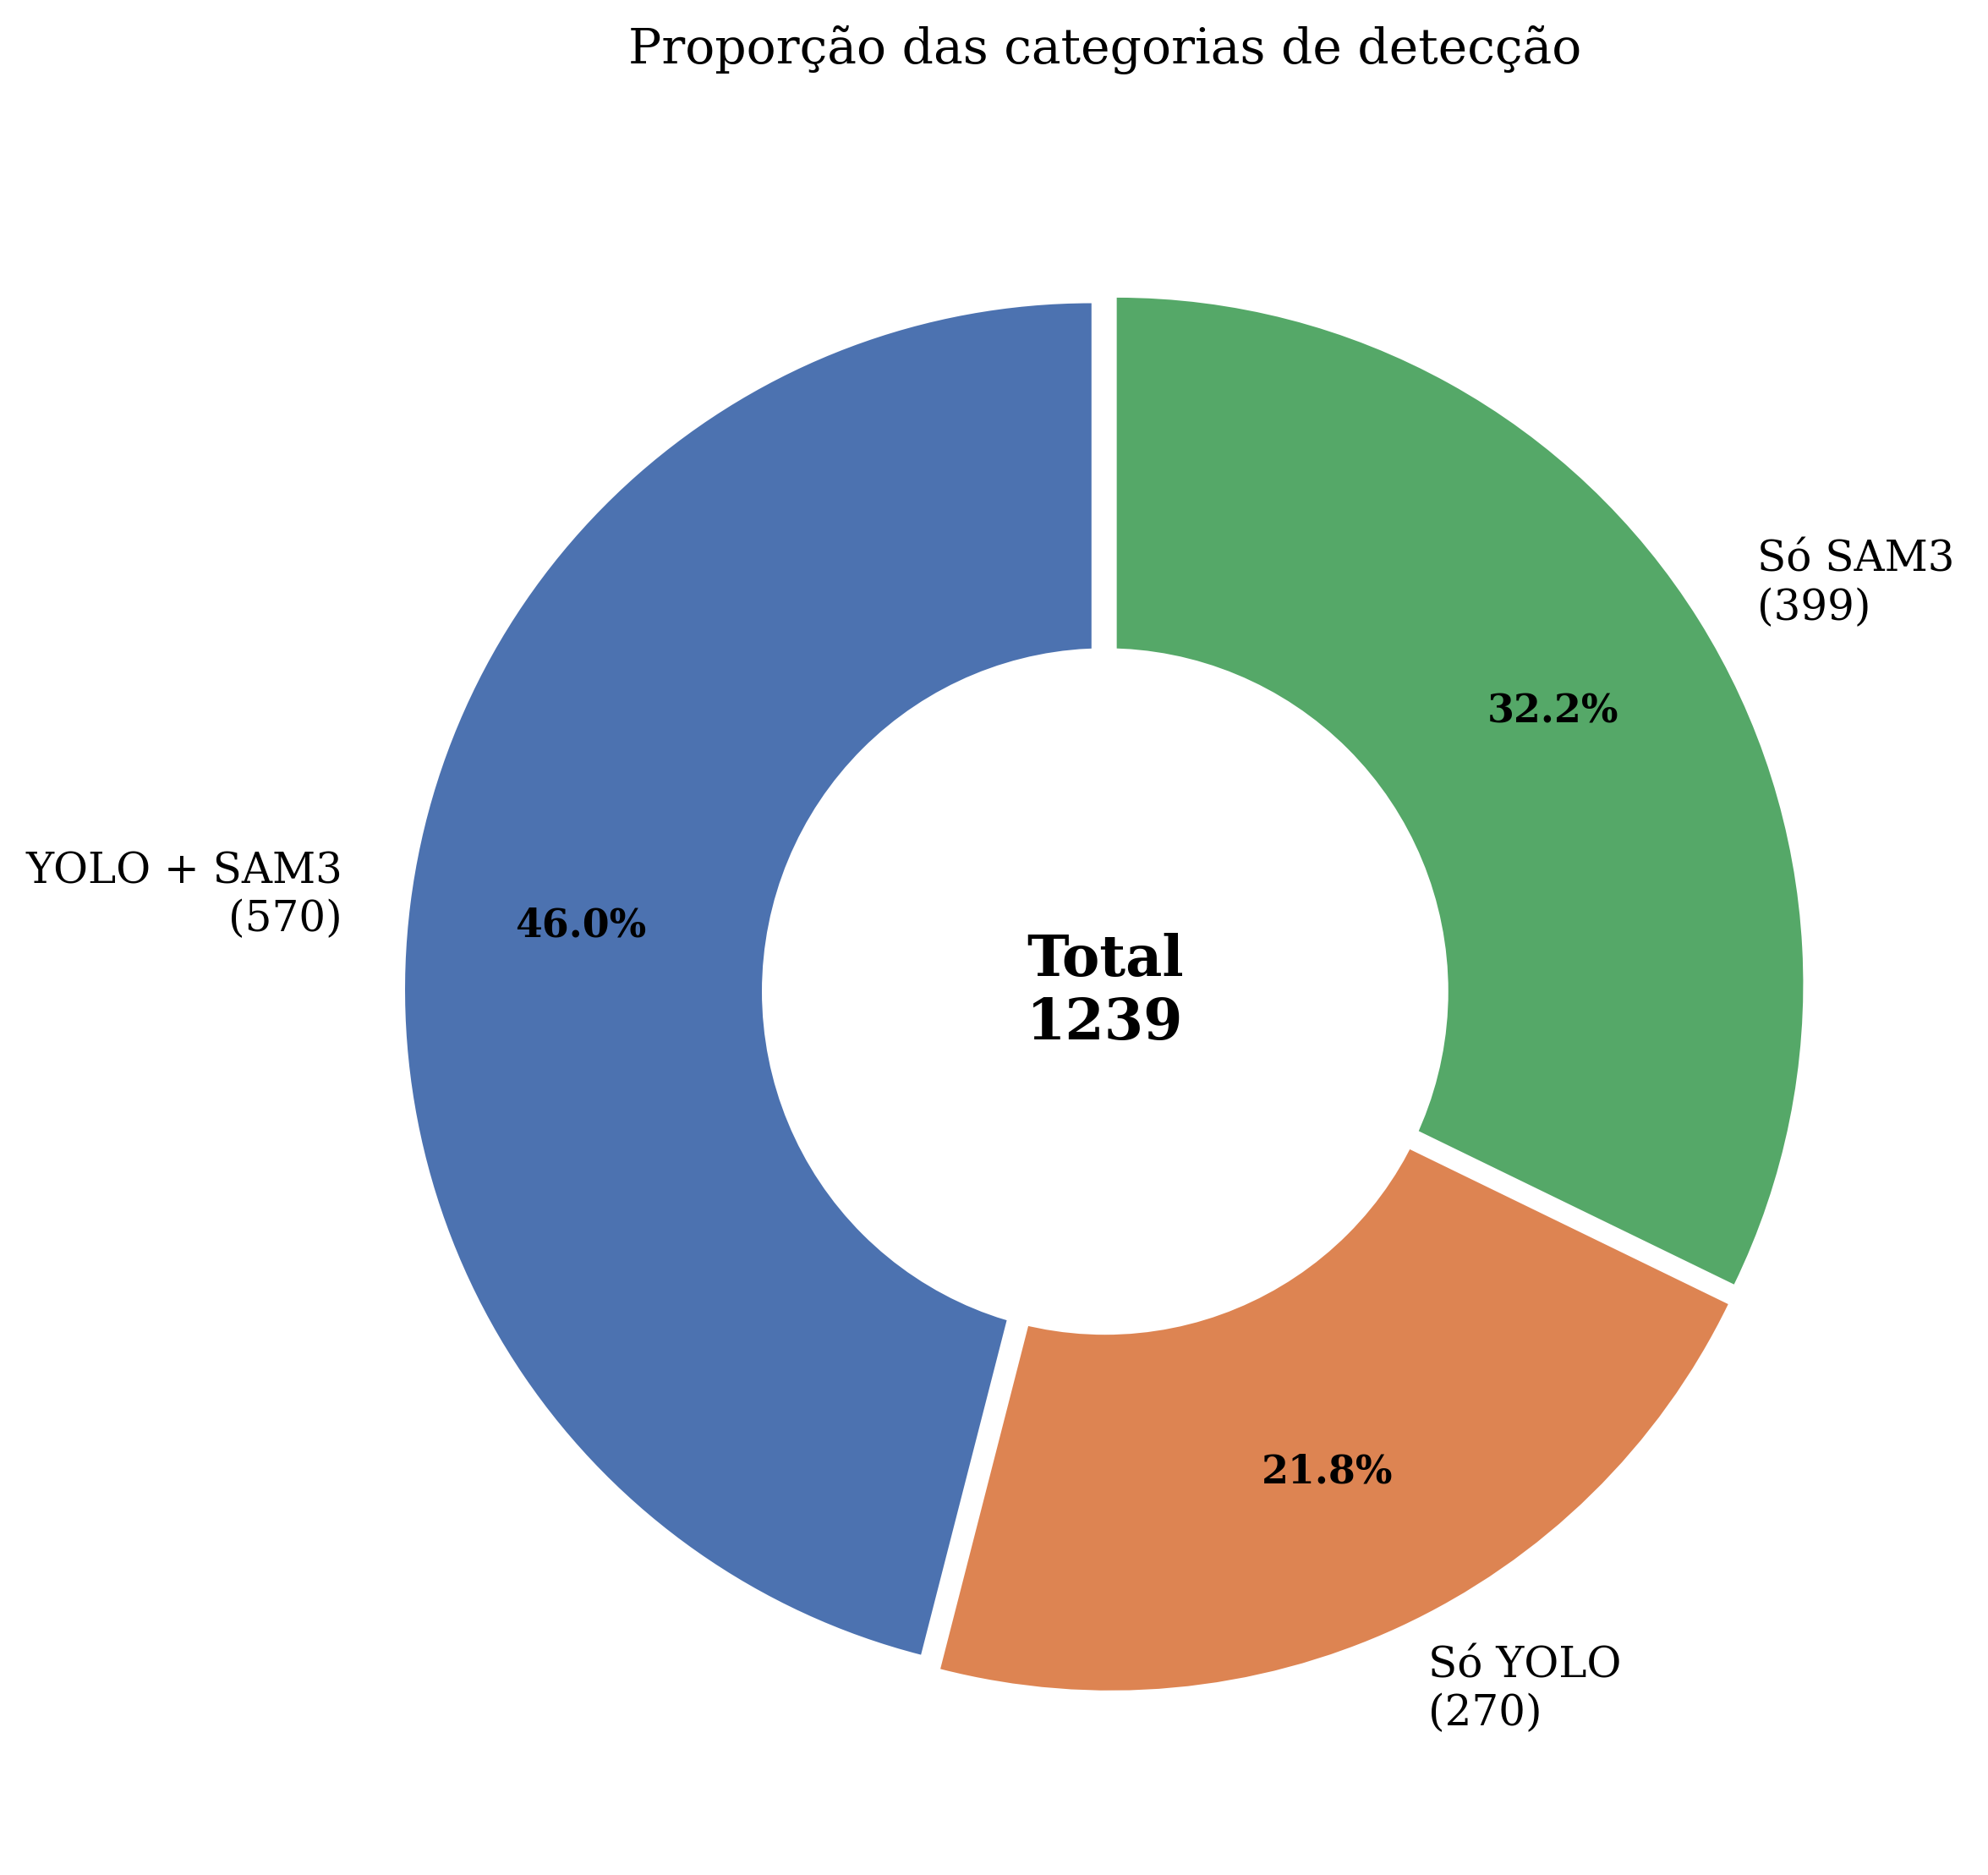
\includegraphics[width=0.82\textwidth]{../rede_neural/figuras/fig06_donut_categorias.png}
    \caption{Proporção das categorias finais do mapeamento neural.}
    \label{fig:neural-donut}
\end{figure}

\subsection{Resultados por composição}

As taxas variaram entre composições. Entre as composições com CP plantada, as
maiores taxas ocorreram em D12 (68,3\%), D7 (65,9\%), D8 (65,7\%) e D11
(62,7\%). A D1, monocultura com 1.200 indivíduos plantados, apresentou 441
indivíduos mapeados e taxa de 36,8\%, sugerindo maior dificuldade em cenário de
copas densas e adjacentes.

\begin{table}[H]
\centering
\caption{Resultados da abordagem neural nas composições com CP plantada.}
\label{tab:neural-composicoes}
\begin{tabular}{lrrrrr}
\toprule
\textbf{Comp.} & \textbf{Parcelas} & \textbf{Plantadas} & \textbf{Mapeadas} & \textbf{Segmentadas} & \textbf{Taxa} \\
\midrule
D1  & 12 & 1.200 & 441 & 442 & 36,8\% \\
D7  & 12 & 396   & 261 & 260 & 65,9\% \\
D8  & 12 & 396   & 260 & 259 & 65,7\% \\
D11 & 12 & 204   & 128 & 129 & 62,7\% \\
D12 & 12 & 60    & 41  & 41  & 68,3\% \\
\bottomrule
\end{tabular}
\end{table}

Também foram mapeados 95 indivíduos em composições sem CP plantada no desenho
experimental. Esses registros devem ser revisados em campo ou por inspeção visual,
pois podem representar indivíduos espontâneos, pequenos deslocamentos entre mapa e
parcelas ou falsos positivos em espécies visualmente semelhantes.

\begin{figure}[H]
    \centering
    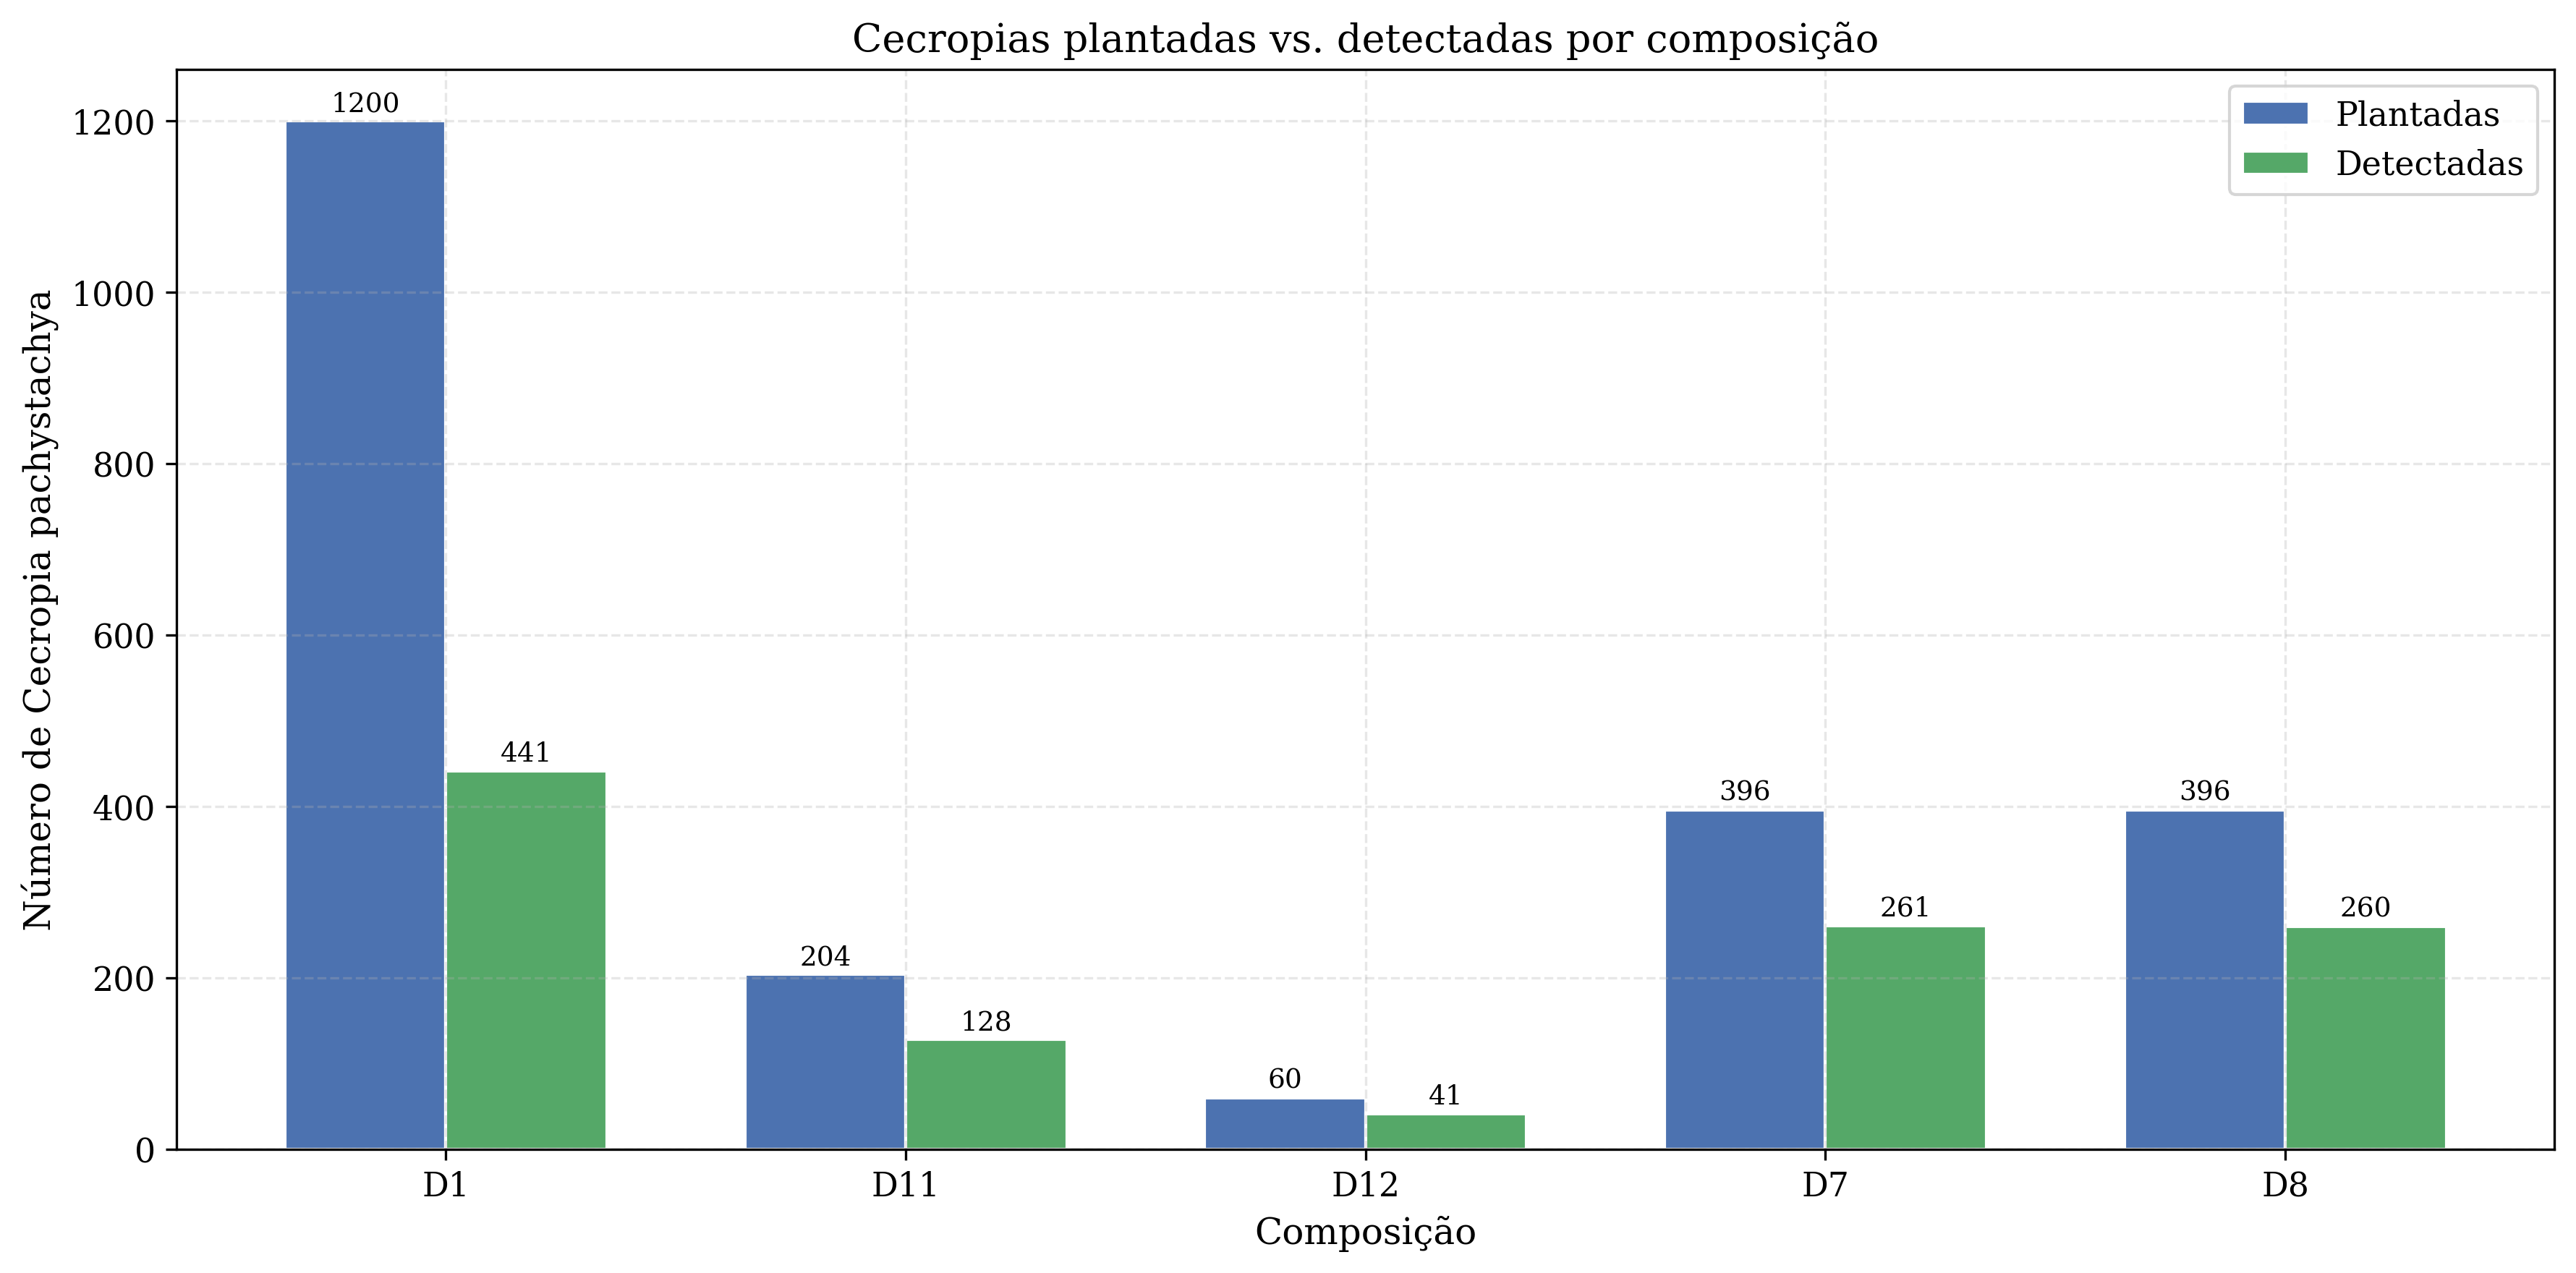
\includegraphics[width=\textwidth]{../rede_neural/figuras/fig01_plantadas_vs_detectadas.png}
    \caption{Indivíduos plantados e mapeados por composição.}
    \label{fig:neural-plantadas-detectadas}
\end{figure}

\begin{figure}[H]
    \centering
    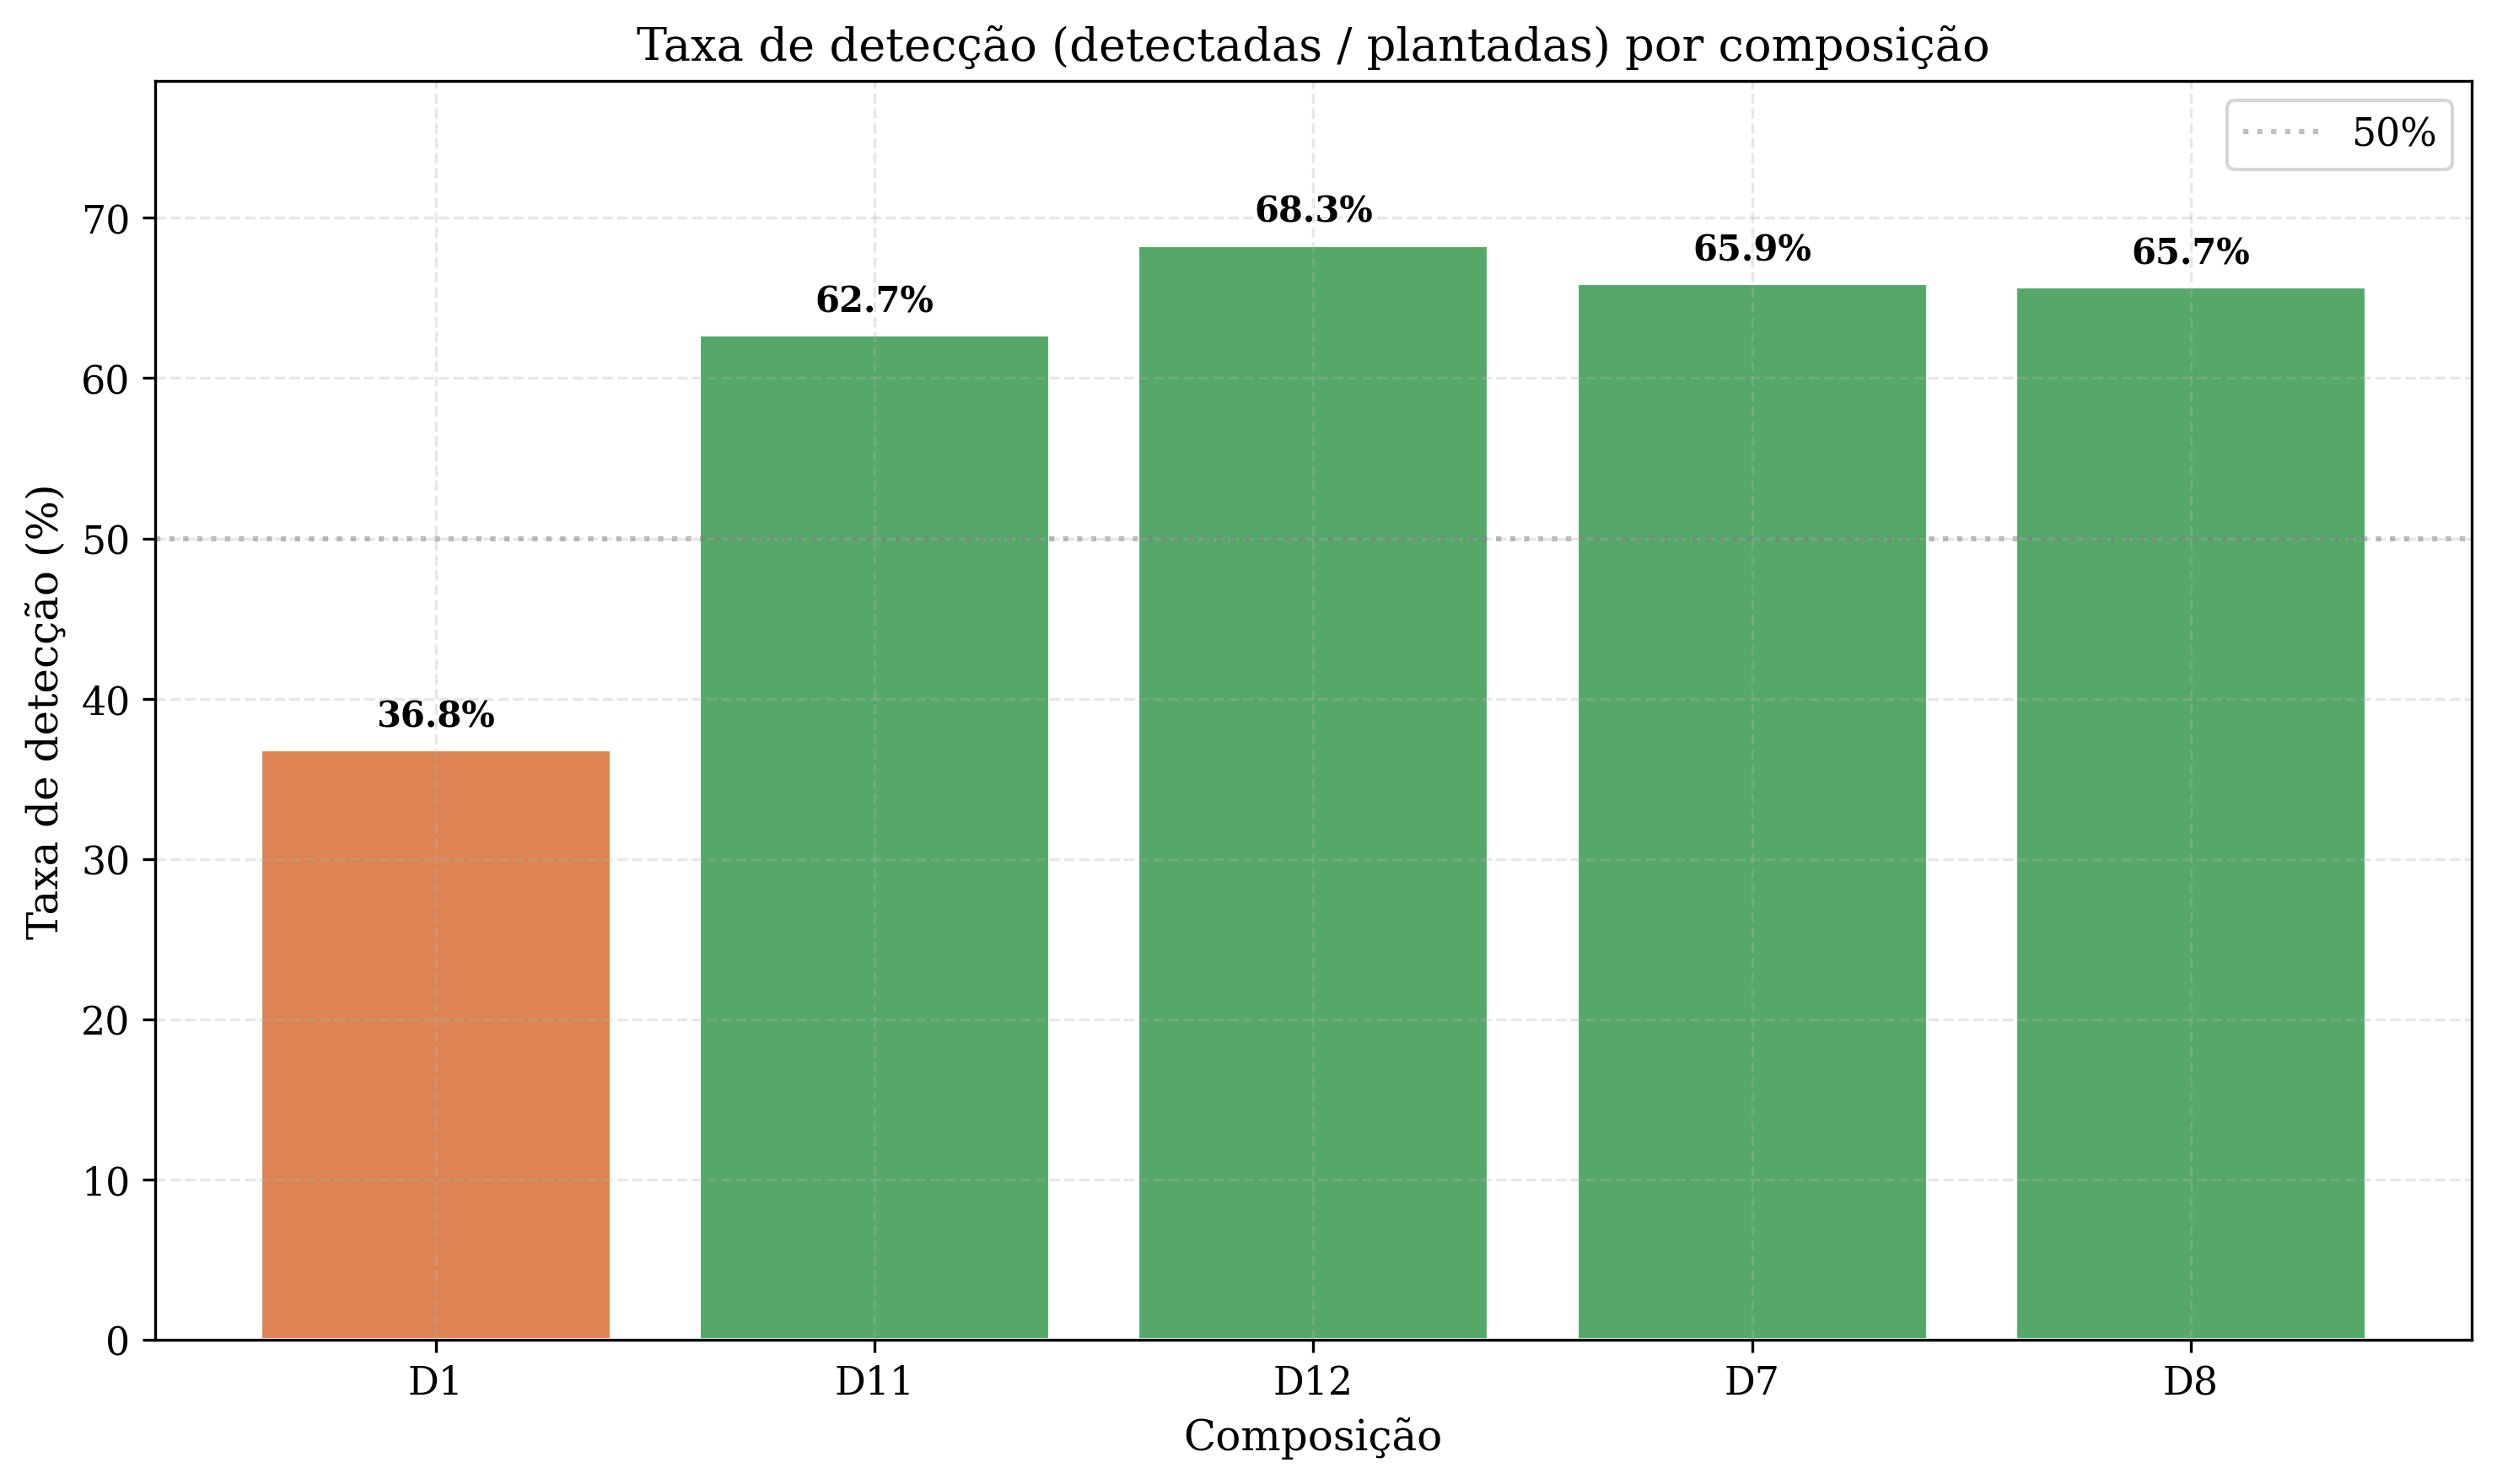
\includegraphics[width=\textwidth]{../rede_neural/figuras/fig05_taxa_deteccao.png}
    \caption{Taxa de detecção por composição.}
    \label{fig:neural-taxa}
\end{figure}

\subsection{Áreas das copas segmentadas}

As 1.228 copas segmentadas apresentaram área média de 5,55 m², mediana de 4,29
m², desvio padrão de 3,93 m² e máximo de 24,26 m². O mínimo arredondado é 0,00
m², mas corresponde no CSV a valor positivo muito pequeno, compatível com
polígonos residuais ou segmentações quase nulas.

\begin{table}[H]
\centering
\caption{Estatísticas de área das copas segmentadas pela abordagem neural.}
\label{tab:neural-areas}
\begin{tabular}{lr}
\toprule
\textbf{Estatística} & \textbf{Valor} \\
\midrule
N copas segmentadas & 1.228 \\
Área média & 5,55 m² \\
Área mediana & 4,29 m² \\
Área mínima & 0,00 m² \\
Área máxima & 24,26 m² \\
Desvio padrão & 3,93 m² \\
\bottomrule
\end{tabular}
\end{table}

As maiores áreas médias ocorreram em D11 (8,11 m²), D8 (7,00 m²) e D6
(6,66 m²). A D1 apresentou média menor (3,86 m²), coerente com maior adensamento
e maior fragmentação visual das copas em monocultura.

\begin{figure}[H]
    \centering
    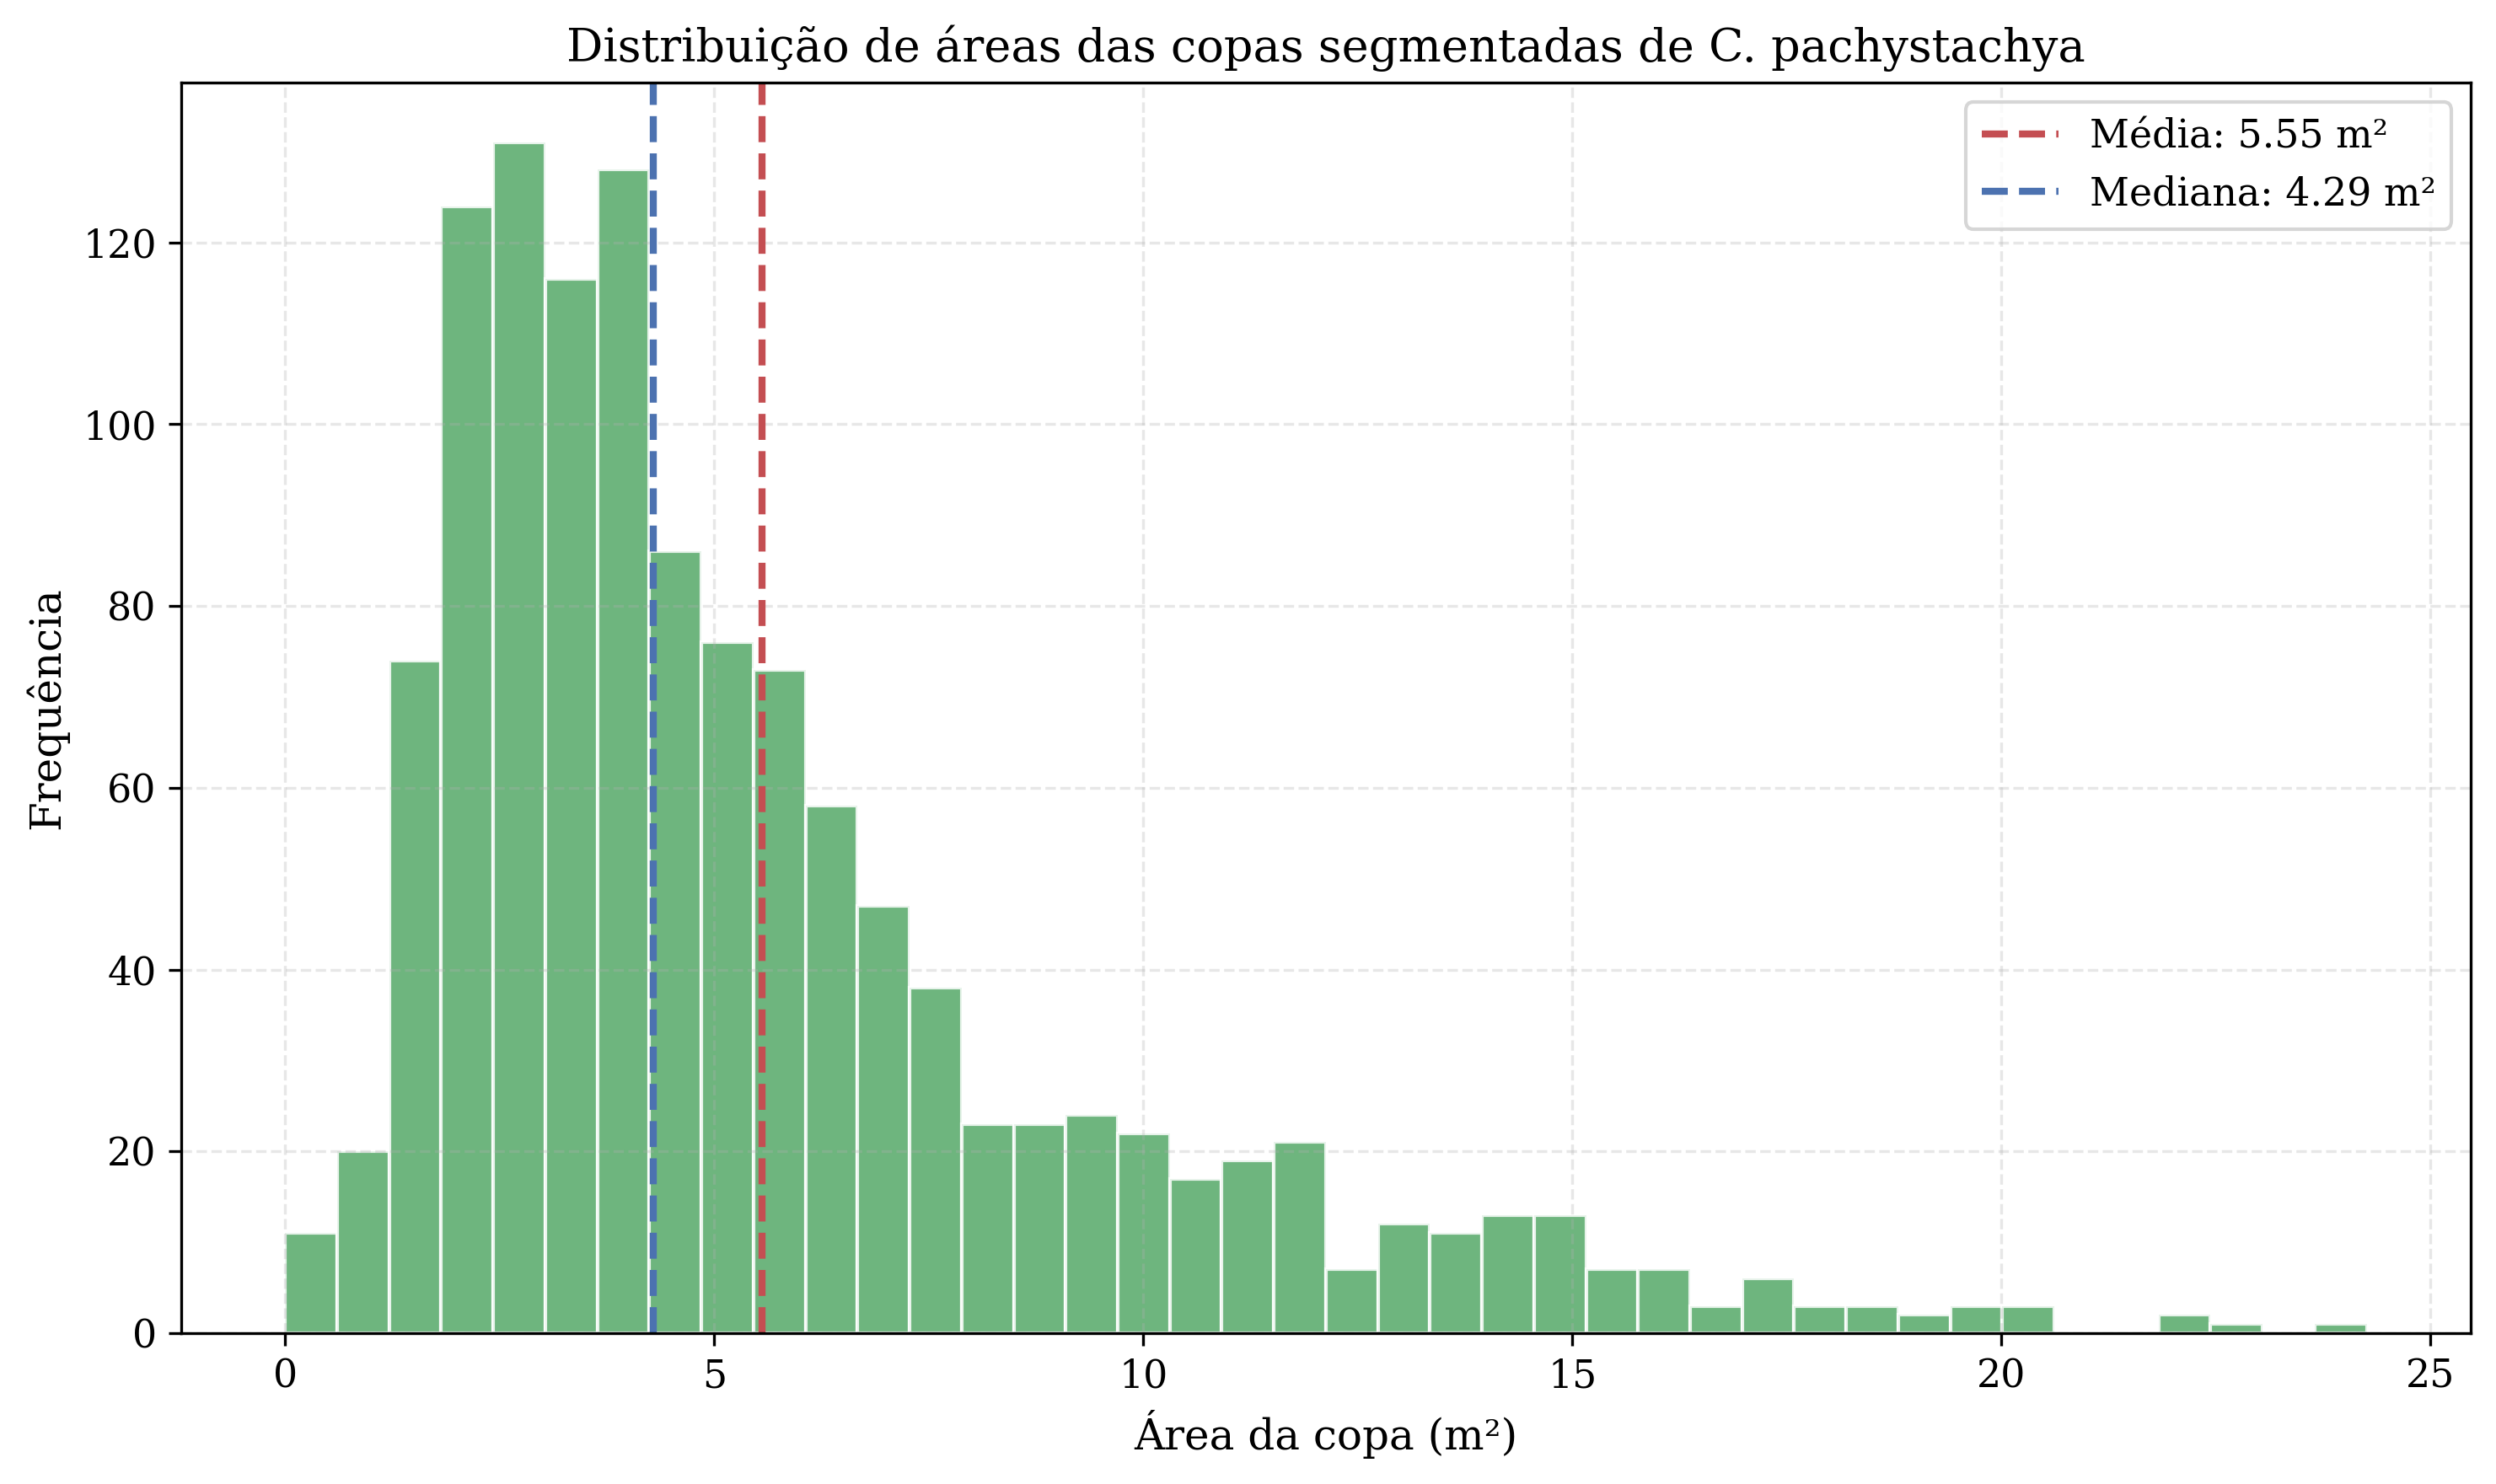
\includegraphics[width=0.86\textwidth]{../rede_neural/figuras/fig03_histograma_areas.png}
    \caption{Distribuição das áreas das copas segmentadas.}
    \label{fig:neural-hist-areas}
\end{figure}

Permanecem pendentes, para a avaliação intrínseca do detector, as métricas de
teste (Precisão, Recall, F1, mAP50 e mAP50-95), as curvas Precision-Recall e de
treino, a importância dos hiperparâmetros e figuras qualitativas sobre o
ortomosaico.

% ═════════════════════════════════════════════════════════════════════════════
\part{Síntese Comparativa}
% ═════════════════════════════════════════════════════════════════════════════

\section{Discussão Comparativa}

As duas abordagens atacam o mesmo problema — mapear copas de \textit{Cecropia
pachystachya} no ortomosaico do MataDIV — por caminhos opostos em termos de
premissas, custo e capacidade de generalização. A Tabela~\ref{tab:comparativo}
resume as principais diferenças.

\begin{table}[H]
\centering
\caption{Comparação entre as duas abordagens.}
\label{tab:comparativo}
\small
\begin{tabular}{p{4.2cm} p{5.2cm} p{5.2cm}}
\toprule
\textbf{Aspecto} & \textbf{Visão Clássica (HSV)} & \textbf{Redes Neurais (SAM 3 + YOLOv8)} \\
\midrule
Sinal explorado & Cor (faixa HSV) e forma (área, circularidade, solidez) & Padrões visuais aprendidos (cor, textura, forma) \\
Anotação & Não requer (revisão manual só para validação) & Curadoria por exclusão sobre máscaras do SAM 3 \\
Interpretabilidade & Alta: cada etapa é auditável & Baixa: decisão distribuída nos pesos da rede \\
Custo computacional & Baixo ($\sim$152 ms/tile, CPU) & Alto (GPU; otimização + treino de 500 épocas) \\
Segmentação de copa & Fecho convexo aproximado & Máscara do SAM 3 (polígono refinado) \\
Discriminação de espécie & Fraca (confusão espectral) & Potencialmente alta (aprende contexto) \\
Resultado & P 86,3\% / R 71,6\% / F1 78,3\% & 1.226 indivíduos mapeados; taxa global 54,3\% \\
\bottomrule
\end{tabular}
\end{table}

A abordagem clássica é leve, transparente e não exige anotação, mas esbarra na
confusão espectral: como diversas espécies caem na mesma faixa de verde, o recall
fica limitado (71,6\%) e há fusão de copas próximas. A abordagem neural procura
justamente superar essa limitação, aprendendo padrões visuais que vão além da cor e
delegando a segmentação fina ao SAM 3. Em contrapartida, exige infraestrutura de
GPU, um ciclo de treinamento longo e uma etapa (ainda que reduzida) de curadoria.

Vale notar que as duas frentes se complementam metodologicamente: o pipeline
clássico funciona como \textit{baseline} interpretável e como ferramenta rápida de
inspeção, enquanto o pipeline neural busca precisão e generalização para outras
espécies. A estratégia de curadoria por exclusão do SAM 3, em particular, reduz
drasticamente a barreira de entrada que normalmente inviabiliza o uso de
aprendizado profundo em contextos botânicos.

\section{Conclusões}

Este trabalho apresentou duas soluções complementares para a detecção e segmentação
de copas de \textit{Cecropia pachystachya} sobre um mesmo ortomosaico de VANT do
experimento MataDIV.

A \textbf{abordagem clássica} (Parte I) demonstrou ser viável para uma primeira
estimativa da distribuição espacial da espécie: é eficiente, escalável por
paralelismo e produz resultados interpretáveis pelas visualizações passo a passo.
Foram detectadas 1.218 regiões em 361 tiles válidos, e a validação manual atingiu
86,3\% de precisão e 71,6\% de recall. O filtro final reduz fortemente os falsos
positivos, mas o recall limitado revela que a dependência de uma faixa HSV fixa
deixa escapar copas reais.

A \textbf{abordagem neural} (Parte II) propõe um pipeline semi-automatizado que
integra o SAM 3 e o YOLOv8, com destaque para a curadoria por exclusão, que reduz o
esforço de anotação, e para a divisão espacial do dataset, que evita vazamento de
dados. A consolidação por parcela mapeou 1.226 indivíduos, segmentou 1.228 copas e
atingiu taxa global de detecção de 54,3\% em relação aos indivíduos plantados. As
maiores taxas ocorreram nas composições D12, D7, D8 e D11, enquanto a D1 mostrou o
maior desafio por densidade e proximidade entre copas.

\subsection*{Trabalhos futuros}

\begin{enumerate}
    \item \textbf{Abordagem clássica:} refinar o intervalo HSV a partir de pixels
    anotados, consolidar detecções entre tiles para evitar contagens repetidas,
    recalibrar os filtros geométricos e incorporar descritores de textura (LBP,
    Haralick) para explorar a estrutura radial das folhas.
    \item \textbf{Abordagem neural:} incorporar métricas formais de teste
    (Precisão, Recall, F1, mAP50 e mAP50-95), revisar detecções em composições sem
    CP plantada e testar a replicabilidade do pipeline para outras espécies
    arbóreas.
    \item \textbf{Integração:} usar o pipeline clássico como pré-filtro rápido e o
    neural como refinamento, ou comparar as duas saídas para estimar incerteza no
    mapeamento final.
\end{enumerate}

\end{document}
